%! Author = loreb
%! Date = 31/10/2023

% Preamble
\documentclass[11pt]{article}

% Packages
\usepackage{amsmath}
\usepackage{graphicx}
\usepackage{float}
\usepackage{csvsimple}
\usepackage{hyperref}
\usepackage{listings}
\usepackage{xcolor}
\usepackage{subcaption}
\usepackage{mdwtab}

\definecolor{codegreen}{rgb}{0,0.6,0}
\definecolor{codegray}{rgb}{0.5,0.5,0.5}
\definecolor{codepurple}{rgb}{0.58,0,0.82}
\definecolor{backcolour}{rgb}{0.95,0.95,0.92}

\lstdefinestyle{mystyle}{
    backgroundcolor=\color{backcolour},
    commentstyle=\color{codegreen},
    keywordstyle=\color{magenta},
    numberstyle=\tiny\color{codegray},
    stringstyle=\color{codepurple},
    basicstyle=\ttfamily\footnotesize,
    breakatwhitespace=false,
    breaklines=true,
    captionpos=b,
    keepspaces=true,
    numbers=left,
    numbersep=5pt,
    showspaces=false,
    showstringspaces=false,
    showtabs=false,
    tabsize=2
}
\lstset{style=mystyle}
\graphicspath{{../results/plots/}}

\title{BloomFilter Speedup on setup and filter: Parallel Programming for Machine Learning}
\author{Lorenzo Baiardi, Thomas Del Moro}
\date{GG MM AAAA}

% Document
\begin{document}

    \maketitle
    \clearpage

    \section{Introduzione}\label{sec:introduzione}
    Il progetto consiste nella parallelizzazione di un BloomFilter per la classificazione di email di spam, utilizzando
    la libreria Omp e Joblib.
    Le operazioni da parallelizzare sono la fase di setup e la fase di filter.
    Vogliamo verificare come varia lo speedup al variare della dimensione dell'insieme su cui effettuare il training,
    come varia lo speedup al variare della numero di processori utilizzati e al variare della implementazione utilizzata.

    \section{Analisi del problema}\label{sec:analisi-del-problema}
    Il BloomFilter è una struttura dati probabilistica che permette di verificare se un elemento appartiene a un insieme,
    in questo caso se un email è di spam o meno.
    La fase di setup del bloom filter consiste nel calcolo delle funzioni hash e nella creazione del vettore di bit che
    si basa sulla dimensione dell'insieme su cui si vuole effettuare il training e sulla probabilità di falsi positivi
    che ci aspettiamo di ottenere.
    La formula per il calcolo della dimensione del vettore di bit è la seguente:
    \begin{equation}
        size = -\frac{n \ln{p}}{(\ln{2})^2}\label{eq:dim_bit}
    \end{equation}
    Dove $size$ è la dimensione del vettore di bit per il training e $n$ è la dimensione dell'insieme che si vuole utilizzare.

    La formula per il calcolo del numero di funzioni hash è la seguente:
    \begin{equation}
        h = \frac{size}{n} \ln{2}\label{eq:num_hash}
    \end{equation}
    Dove $h$ è il numero di funzioni hash da utilizzare per il training.

    Una volta passato il dataset di training al bloom filter, questo calcola per ogni email le $h$ funzioni hash e setta
    a 1 i bit corrispondenti alle posizioni calcolate.
    Per verificare se un email è di spam o meno, il bloom filter calcola le $h$ funzioni hash e verifica se i bit
    corrispondenti alle posizioni calcolate sono settati a 1.

    \section{Parallelizzazione}\label{sec:parallelizazzione}
    Il codice sequenziale di riferimento da parallelizzare per la fase di setup è il seguente:
    \lstinputlisting[language=python, firstline=33, lastline=39,label={lst:sequential-code-setup-joblib}]{../src/bloom_filter.py}
    \lstinputlisting[language=c++, firstline=22, lastline=28,label={lst:sequential-code-setup-omp}]{references/BloomFilter.cpp}

    Il codice sequenziale di riferimento da parallelizzare per la fase di filter è il seguente:
    \lstinputlisting[language=python, firstline=58, lastline=66,label={lst:sequential-code-filter-joblib}]{../src/bloom_filter.py}
    \lstinputlisting[language=c++, firstline=45, lastline=51,label={lst:sequential-code-filter-omp}]{references/BloomFilter.cpp}

    \subsection{Omp}\label{subsec:omp}
    Omp è una libreria C che permette di parallelizzare funzioni e cicli for.
    La funzione omp parallel prende in input il numero di processori da utilizzare e la funzione da parallelizzare.
    In questo elaborato abbiamo utilizzato la funzione omp parallel for per parallelizzare la funzione setup e la
    funzione filter del bloom filter.
    Abbiamo poi successivamente elaborato quanto tempo impiegano le funzioni setup e filter a seconda del numero di
    processori utilizzati rispetto al tempo impiegato nella sua versione sequenziale.
    \lstinputlisting[language=c++, firstline=30, lastline=37, label={lst:sequential-code}]{references/BloomFilter.cpp}

    \subsection{Joblib}\label{subsec:joblib}
    Joblib è una libreria Python che permette di parallelizzare funzioni e cicli for.
    La funzione Parallel prende in input il numero di processori da utilizzare e la funzione da parallelizzare.
    In questo elaborato abbiamo utilizzato la funzione Parallel per parallelizzare la funzione setup e la funzione
    filter del bloom filter.
    Abbiamo poi successivamente elaborato quanto tempo impiegano le funzioni setup e filter a seconda del numero di
    processori utilizzati rispetto al tempo impiegato nella sua versione sequenziale.
    \lstinputlisting[language=python, firstline=41, lastline=50,label={lst:joblib-code-setup}]{../src/bloom_filter.py}
    \lstinputlisting[language=python, firstline=68, lastline=80,label={lst:joblib-code-filter}]{../src/bloom_filter.py}

    \section{Caratteristiche della macchina}\label{sec:caratteristiche-della-macchina}
    La macchina utilizzata per i test ha le seguenti caratteristiche:
    \begin{itemize}
        \item \textbf{CPU}: Intel Core i7-1360P (4 P-Core, 8 E-Core, 12 Cores, 16 Threads)
        \item \textbf{RAM}: 16GB
        \item \textbf{Sistema Operativo}: Windows 11
    \end{itemize}

    \section{Tests}\label{sec:tests}
    I test sono stati effettuati su un dataset da 1000 fino a 10000000 email, con una probabilità di falsi positivi che
    varia da 0.10 a 0.01.

    \section{Risultati}\label{sec:risultati}
    \subsection{FPR: 0.10}\label{subsec:fpr-010}
    \subsubsection{Setup}\label{subsubsec:fpr-010-setup}
    \begin{figure}[H]
        \centering
        \minipage{0.49\textwidth}
        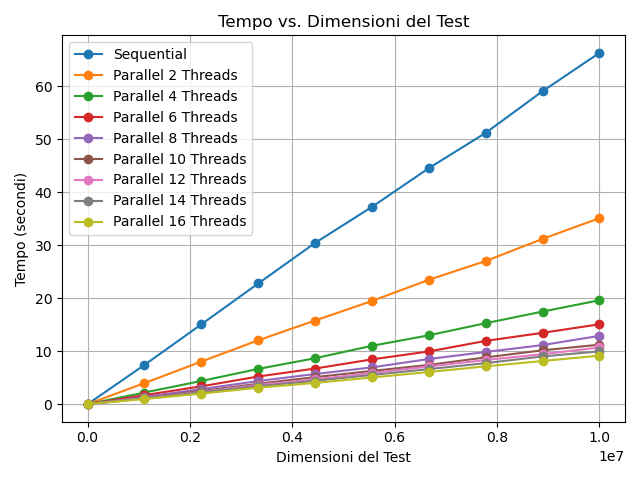
\includegraphics[width=\linewidth]{omp/010/setup_time_plot}
            \caption{Speedup setup Omp}\label{fig:010-setup_time_omp}
        \endminipage\hfill
        \minipage{0.49\textwidth}
        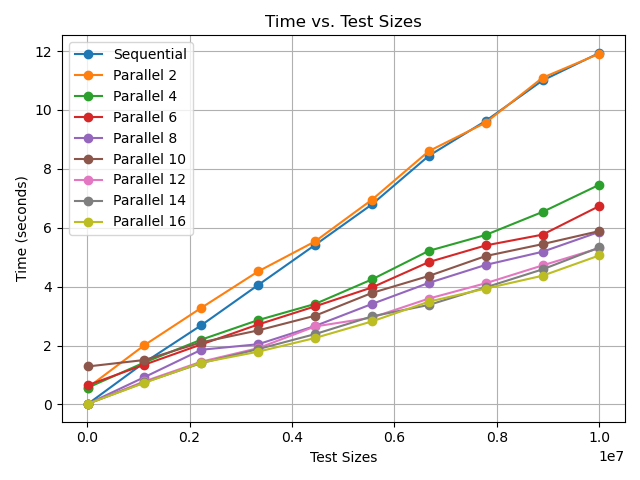
\includegraphics[width=\linewidth]{joblib/010/setup_time_plot}
            \caption{Speedup setup Joblib}\label{fig:010setup_time_joblib}
        \endminipage\hfill
        \caption{Time setup}
    \end{figure}
    \begin{figure}[H]
        \centering
        \minipage{0.49\textwidth}
        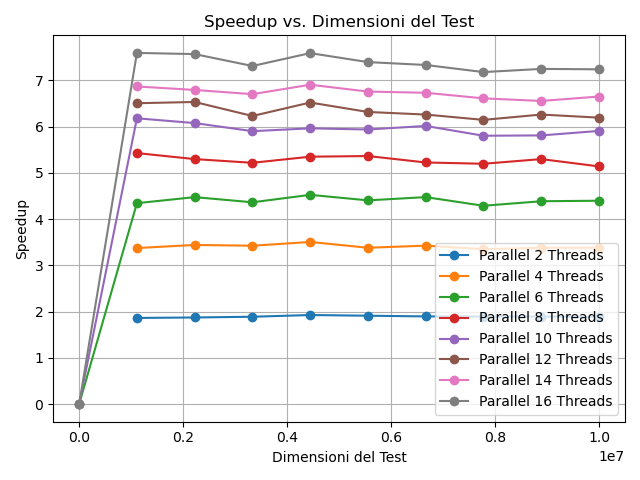
\includegraphics[width=\linewidth]{omp/010/setup_speedup_plot}
            \caption{Speedup setup Omp}\label{fig:010-setup_speedup_omp}
        \endminipage\hfill
        \minipage{0.49\textwidth}
        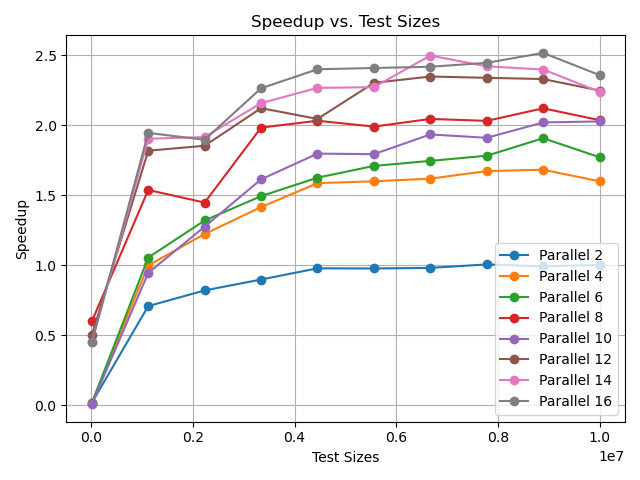
\includegraphics[width=\linewidth]{joblib/010/setup_speedup_plot}
            \caption{Speedup setup Joblib}\label{fig:010-setup_speedup_joblib}
        \endminipage\hfill
        \caption{Speedup setup}
    \end{figure}
    \begin{figure}[H]
        \centering
        \minipage{0.49\textwidth}
        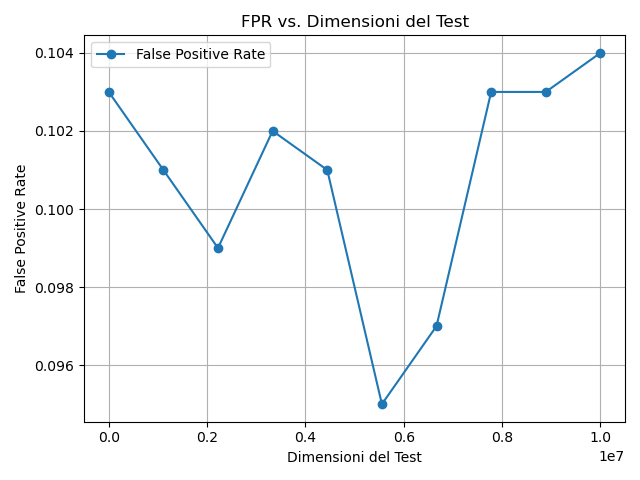
\includegraphics[width=\linewidth]{omp/010/setup_fpr_plot}
            \caption{Speedup setup Omp}\label{fig:010-setup_fpr_omp}
        \endminipage\hfill
        \minipage{0.49\textwidth}
        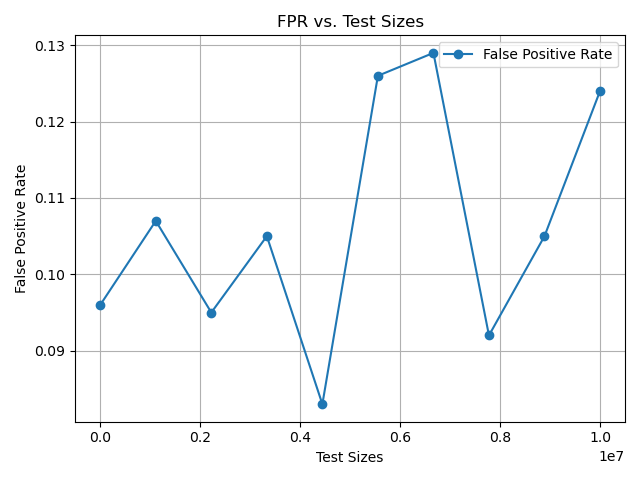
\includegraphics[width=\linewidth]{joblib/010/setup_fpr_plot}
            \caption{Speedup setup Joblib}\label{fig:010-setup_fpr_joblib}
        \endminipage\hfill
        \caption{Time setup}
    \end{figure}
    \subsubsection{Filter}\label{subsubsec:fpr-010-filter}
    \begin{figure}[H]
        \centering
        \minipage{0.49\textwidth}
        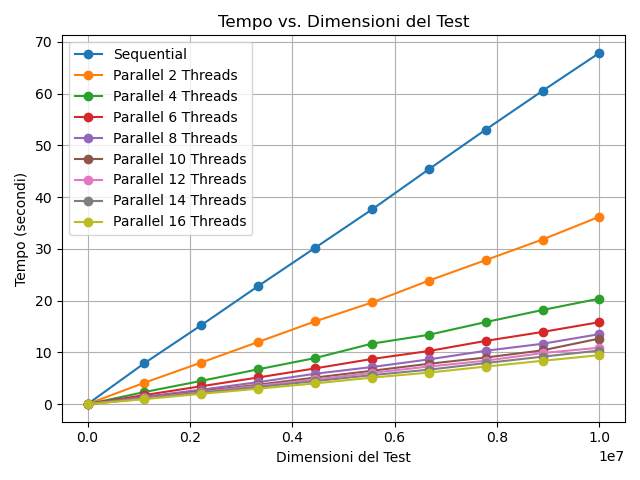
\includegraphics[width=\linewidth]{omp/010/filter_time_plot}
            \caption{Speedup setup Omp}\label{fig:010-filter_time_omp}
        \endminipage\hfill
        \minipage{0.49\textwidth}
        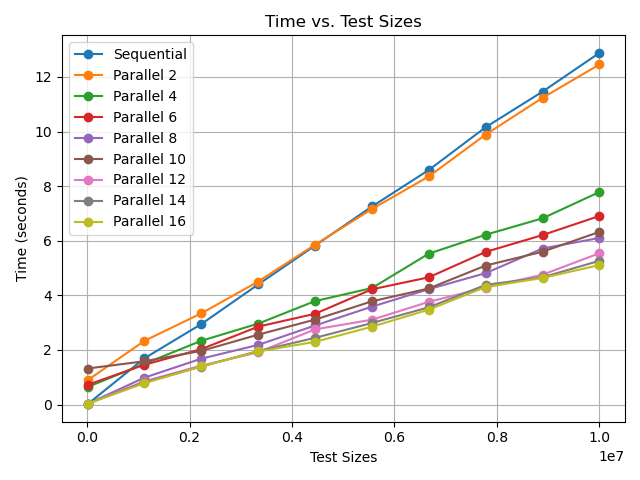
\includegraphics[width=\linewidth]{joblib/010/filter_time_plot}
            \caption{Speedup setup Joblib}\label{fig:010-filter_time_joblib}
        \endminipage\hfill
        \caption{Time setup}
    \end{figure}
    \begin{figure}[H]
        \centering
        \minipage{0.49\textwidth}
        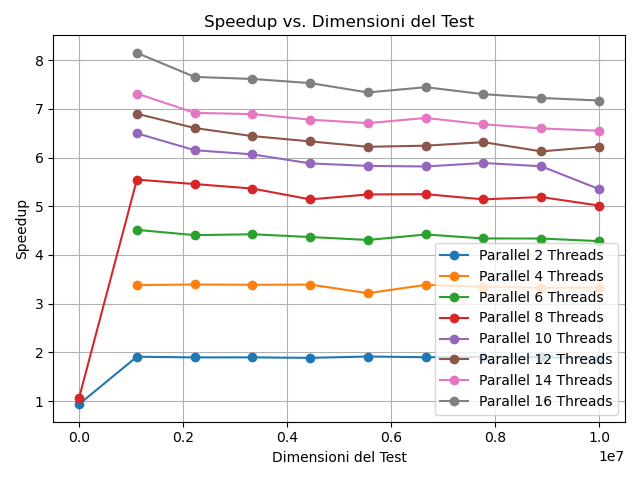
\includegraphics[width=\linewidth]{omp/010/filter_speedup_plot}
            \caption{Speedup setup Omp}\label{fig:010-filter_speedup_omp}
        \endminipage\hfill
        \minipage{0.49\textwidth}
        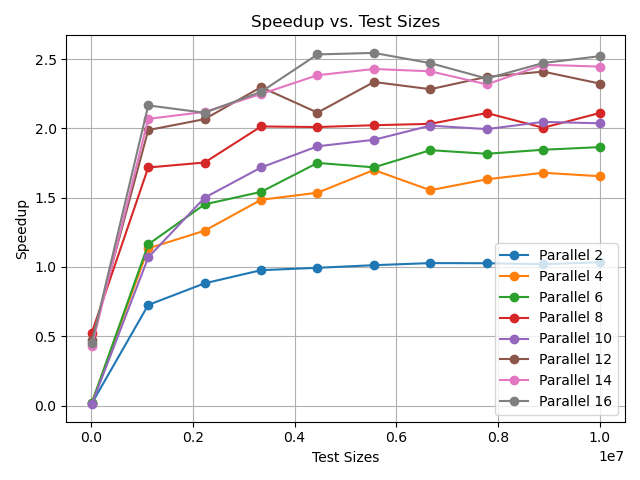
\includegraphics[width=\linewidth]{joblib/010/filter_speedup_plot}
            \caption{Speedup setup Joblib}\label{fig:010-filter_speedup_joblib}
        \endminipage\hfill
        \caption{Speedup setup}
    \end{figure}
    \begin{figure}[H]
        \centering
        \minipage{0.49\textwidth}
        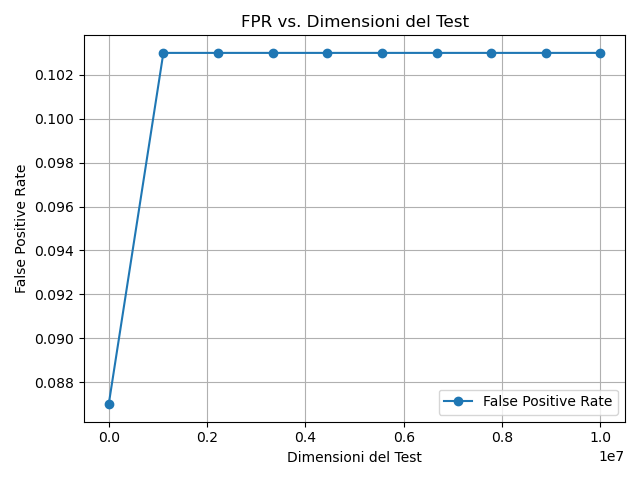
\includegraphics[width=\linewidth]{omp/010/filter_fpr_plot}
            \caption{Speedup setup Omp}\label{fig:010-filter_fpr_omp}
        \endminipage\hfill
        \minipage{0.49\textwidth}
        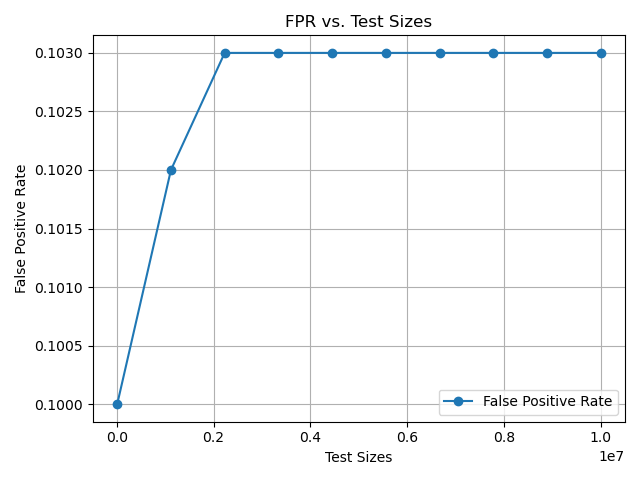
\includegraphics[width=\linewidth]{joblib/010/filter_fpr_plot}
            \caption{Speedup setup Joblib}\label{fig:010-filter_fpr_joblib}
        \endminipage\hfill
        \caption{Time setup}
    \end{figure}
    \subsubsection{Chunks}\label{subsubsec:010-chunks}
    \begin{figure}[H]
        \centering
        \minipage{0.49\textwidth}
        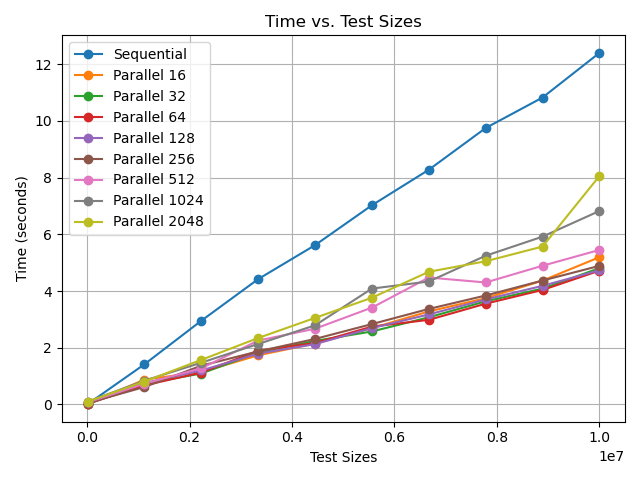
\includegraphics[width=\linewidth]{joblib/010/chunks_time_plot}
            \caption{Times setup Chunk}\label{fig:010-chunks_time}
        \endminipage\hfill
        \minipage{0.49\textwidth}
        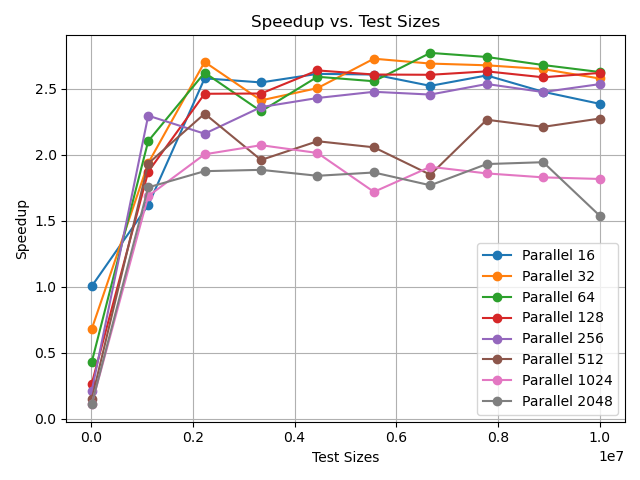
\includegraphics[width=\linewidth]{joblib/010/chunks_speedup_plot}
            \caption{Speedup setup Chunk}\label{fig:010-chunks_speedup}
        \endminipage\hfill
        \caption{Time setup}
    \end{figure}

    \subsection{FPR: 0.05}\label{subsec:fpr-005}
    \subsubsection{Setup}\label{subsubsec:fpr-005-setup}
    \begin{figure}[H]
        \centering
        \minipage{0.49\textwidth}
        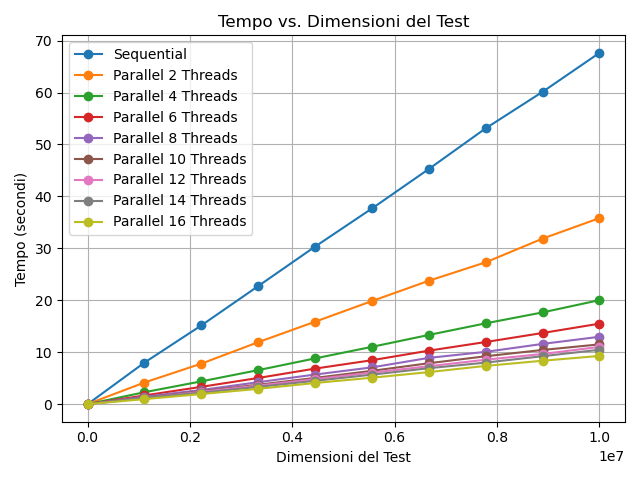
\includegraphics[width=\linewidth]{omp/005/setup_time_plot}
            \caption{Speedup setup Omp}\label{fig:005-setup_time_omp}
        \endminipage\hfill
        \minipage{0.49\textwidth}
        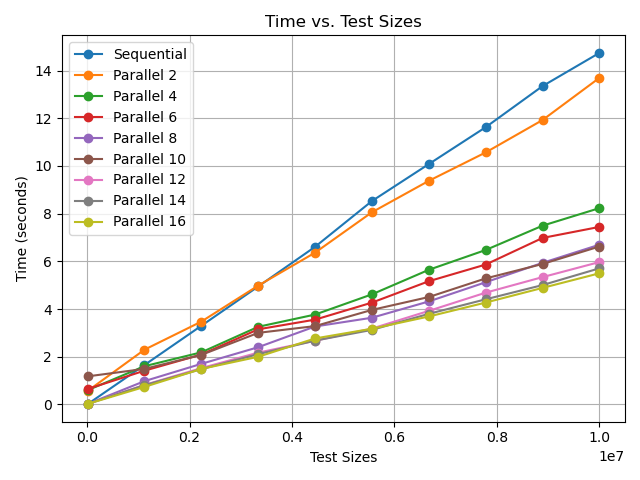
\includegraphics[width=\linewidth]{joblib/005/setup_time_plot}
            \caption{Speedup setup Joblib}\label{fig:005-setup_time_joblib}
        \endminipage\hfill
        \caption{Time setup}
    \end{figure}
    \begin{figure}[H]
        \centering
        \minipage{0.49\textwidth}
        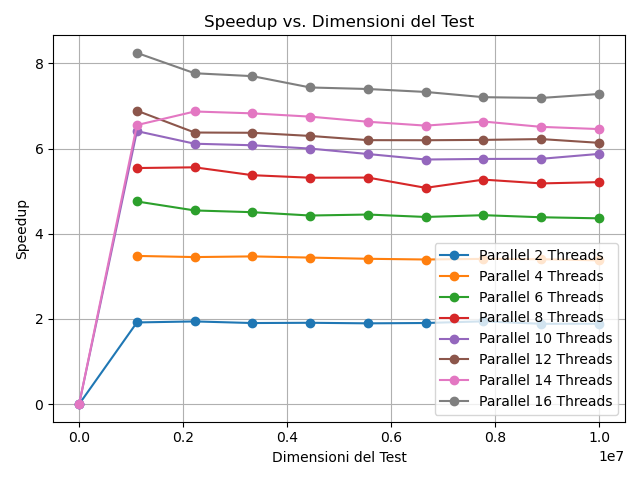
\includegraphics[width=\linewidth]{omp/005/setup_speedup_plot}
            \caption{Speedup setup Omp}\label{fig:005-setup_speedup_omp}
        \endminipage\hfill
        \minipage{0.49\textwidth}
        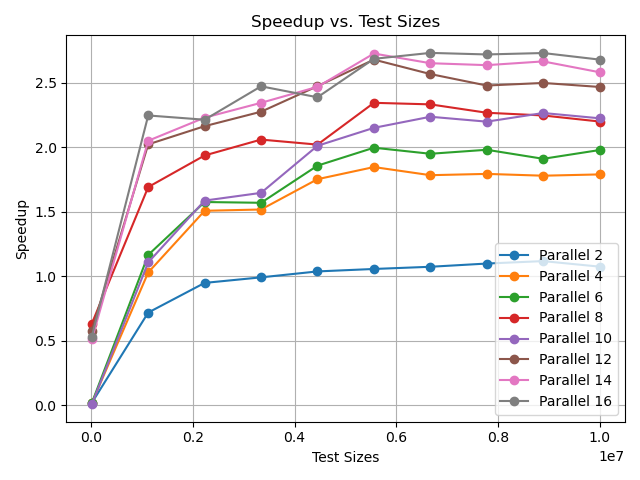
\includegraphics[width=\linewidth]{joblib/005/setup_speedup_plot}
            \caption{Speedup setup Joblib}\label{fig:005-setup_speedup_joblib}
        \endminipage\hfill
        \caption{Speedup setup}
    \end{figure}
    \begin{figure}[H]
        \centering
        \minipage{0.49\textwidth}
        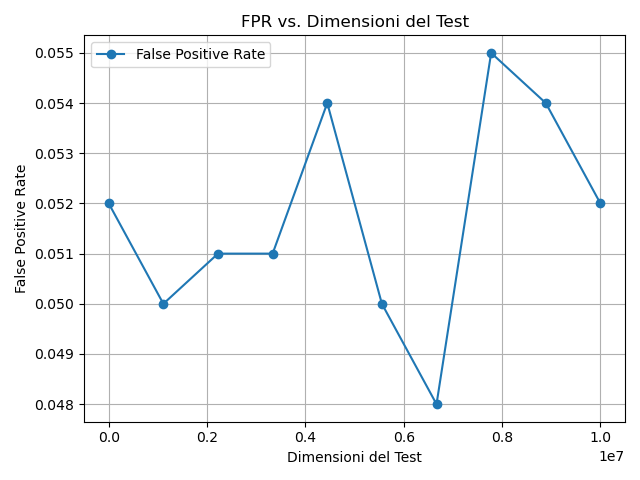
\includegraphics[width=\linewidth]{omp/005/setup_fpr_plot}
            \caption{Speedup setup Omp}\label{fig:005-setup_fpr_omp}
        \endminipage\hfill
        \minipage{0.49\textwidth}
        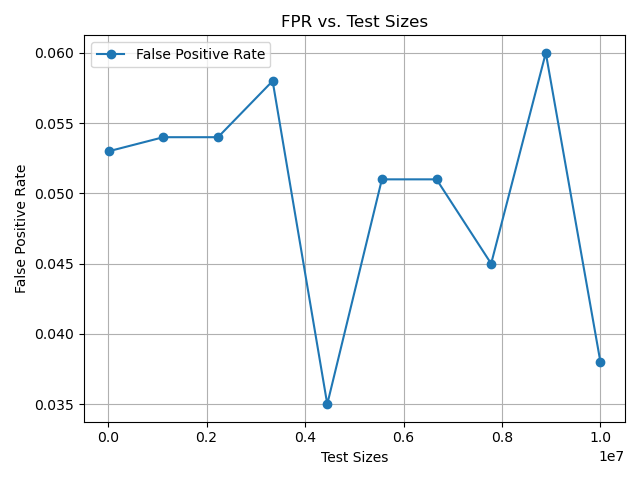
\includegraphics[width=\linewidth]{joblib/005/setup_fpr_plot}
            \caption{Speedup setup Joblib}\label{fig:005-setup_fpr_joblib}
        \endminipage\hfill
        \caption{Time setup}
    \end{figure}
    \subsubsection{Filter}\label{subsubsec:fpr-005-filter}
    \begin{figure}[H]
        \centering
        \minipage{0.49\textwidth}
        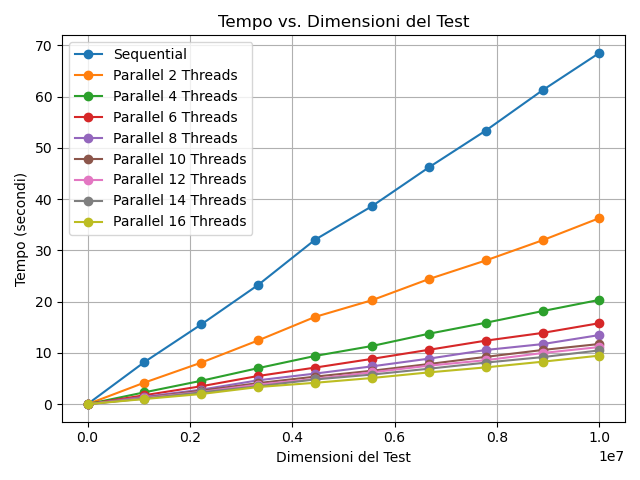
\includegraphics[width=\linewidth]{omp/005/filter_time_plot}
            \caption{Speedup setup Omp}\label{fig:005-filter_time_omp}
        \endminipage\hfill
        \minipage{0.49\textwidth}
        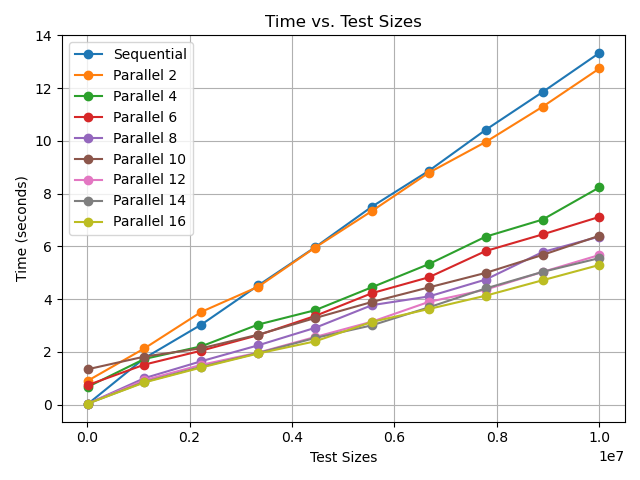
\includegraphics[width=\linewidth]{joblib/005/filter_time_plot}
            \caption{Speedup setup Joblib}\label{fig:005-filter_time_joblib}
        \endminipage\hfill
        \caption{Time setup}
    \end{figure}
    \begin{figure}[H]
        \centering
        \minipage{0.49\textwidth}
        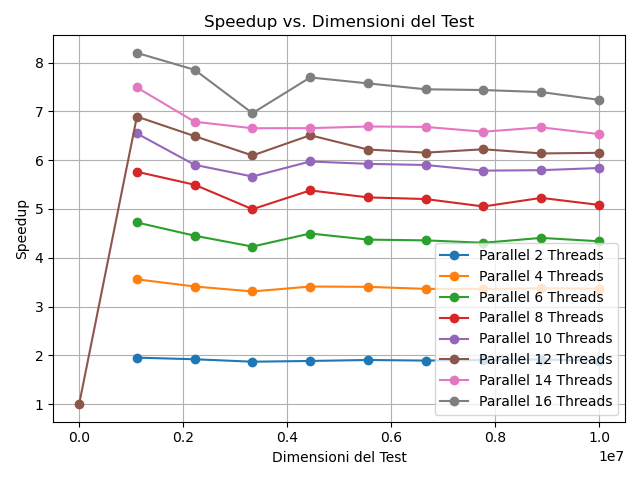
\includegraphics[width=\linewidth]{omp/005/filter_speedup_plot}
            \caption{Speedup setup Omp}\label{fig:005-filter_speedup_omp}
        \endminipage\hfill
        \minipage{0.49\textwidth}
        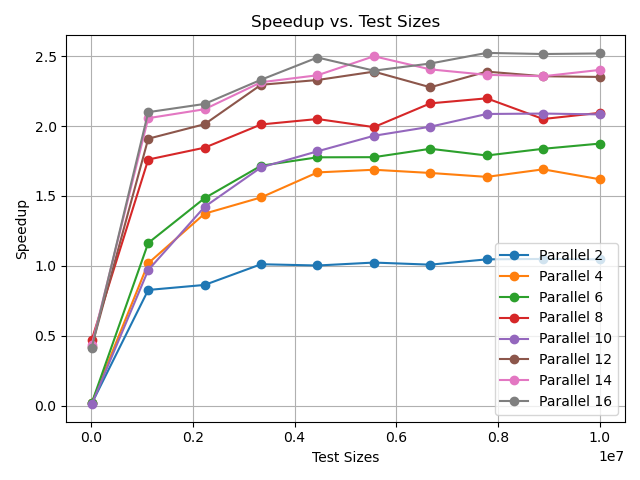
\includegraphics[width=\linewidth]{joblib/005/filter_speedup_plot}
            \caption{Speedup setup Joblib}\label{fig:005-filter_speedup_joblib}
        \endminipage\hfill
        \caption{Speedup setup}
    \end{figure}
    \begin{figure}[H]
        \centering
        \minipage{0.49\textwidth}
        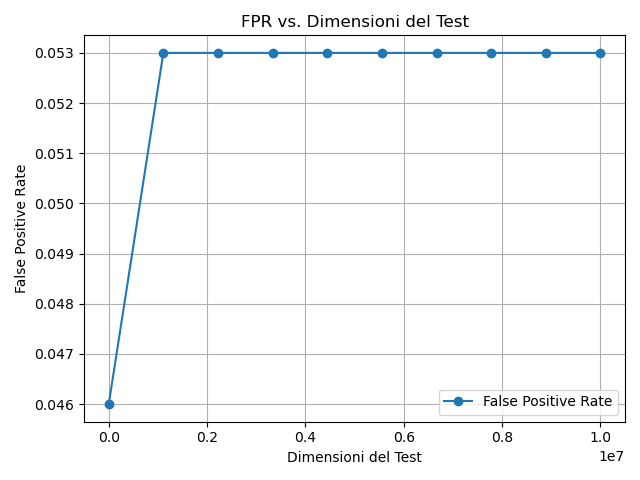
\includegraphics[width=\linewidth]{omp/005/filter_fpr_plot}
            \caption{Speedup setup Omp}\label{fig:005-filter_fpr_omp}
        \endminipage\hfill
        \minipage{0.49\textwidth}
        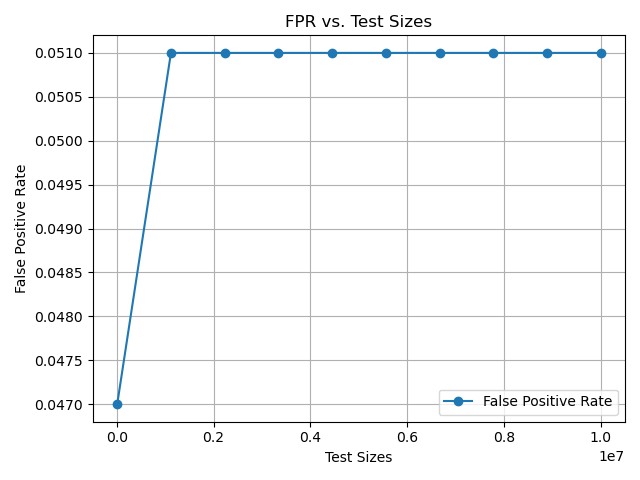
\includegraphics[width=\linewidth]{joblib/005/filter_fpr_plot}
            \caption{Speedup setup Joblib}\label{fig:005-filter_fpr_joblib}
        \endminipage\hfill
        \caption{Time setup}
    \end{figure}
    \subsubsection{Chunks}\label{subsubsec:005-chunks}
    \begin{figure}[H]
        \centering
        \minipage{0.49\textwidth}
        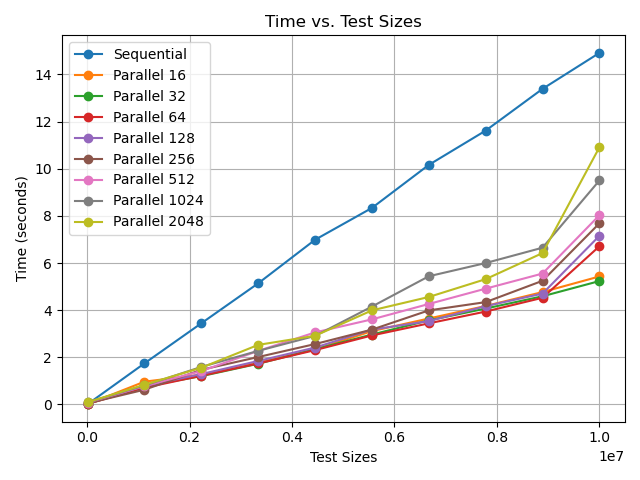
\includegraphics[width=\linewidth]{joblib/005/chunks_time_plot}
            \caption{TImes setup Chunks}\label{fig:005-chunks_time}
        \endminipage\hfill
        \minipage{0.49\textwidth}
        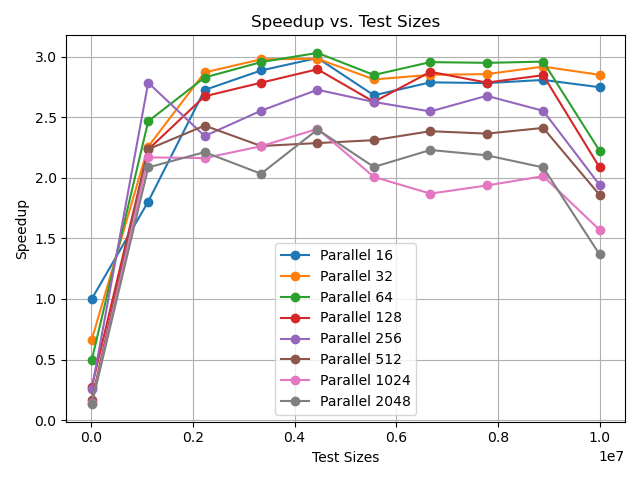
\includegraphics[width=\linewidth]{joblib/005/chunks_speedup_plot}
            \caption{Speedup setup Chunks}\label{fig:005-chunks_speedup}
        \endminipage\hfill
        \caption{Time setup}
    \end{figure}

    \subsection{FPR: 0.01}\label{subsec:fpr-001}
    \subsubsection{Setup}\label{subsubsec:setup}
    \begin{figure}[H]
        \centering
        \minipage{0.49\textwidth}
        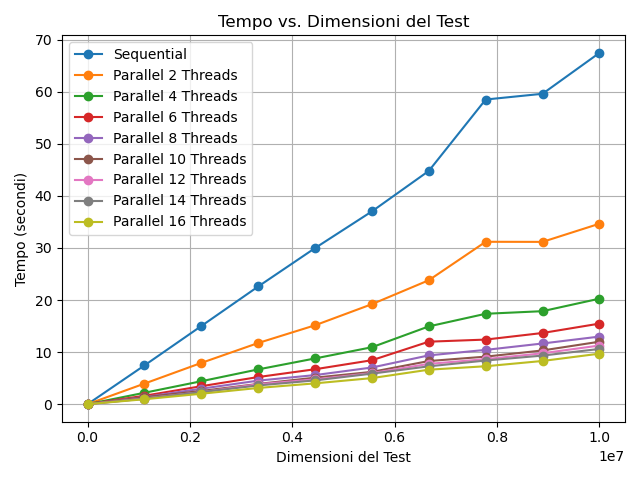
\includegraphics[width=\linewidth]{omp/001/setup_time_plot}
            \caption{Speedup setup Omp}\label{fig:setup_time_omp}
        \endminipage\hfill
        \minipage{0.49\textwidth}
        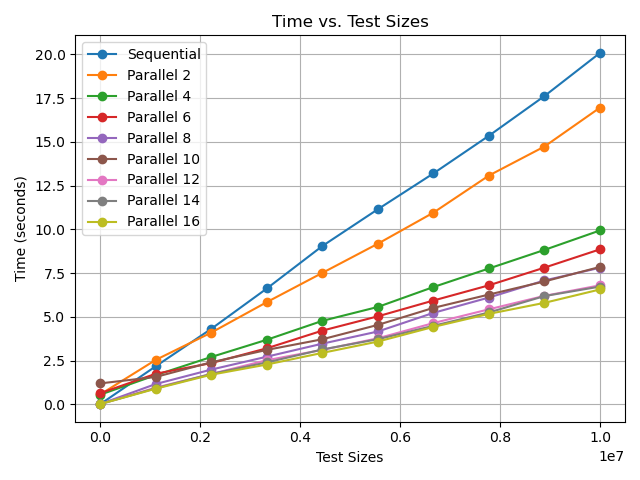
\includegraphics[width=\linewidth]{joblib/001/setup_time_plot}
            \caption{Speedup setup Joblib}\label{fig:setup_time_joblib}
        \endminipage\hfill
        \caption{Time setup}
    \end{figure}
    \begin{figure}[H]
        \centering
        \minipage{0.49\textwidth}
        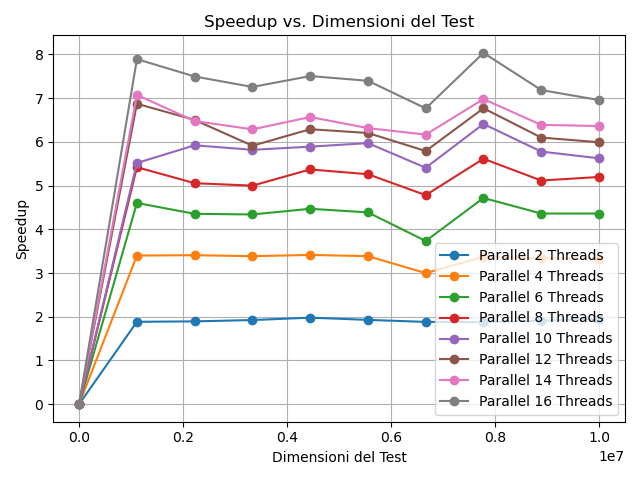
\includegraphics[width=\linewidth]{omp/001/setup_speedup_plot}
            \caption{Speedup setup Omp}\label{fig:setup_speedup_omp}
        \endminipage\hfill
        \minipage{0.49\textwidth}
        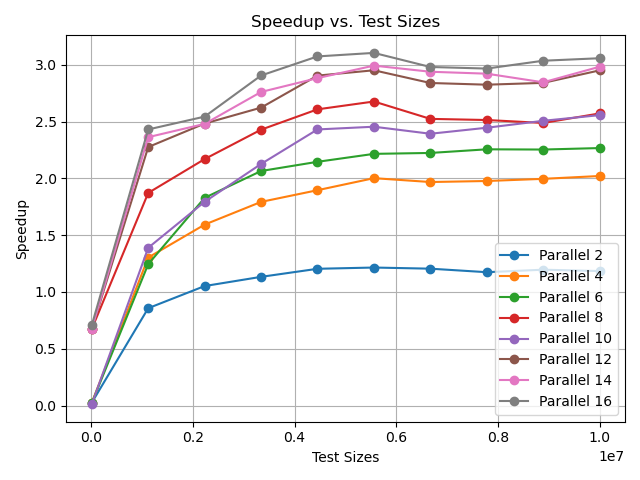
\includegraphics[width=\linewidth]{joblib/001/setup_speedup_plot}
            \caption{Speedup setup Joblib}\label{fig:setup_speedup_joblib}
        \endminipage\hfill
        \caption{Speedup setup}
    \end{figure}
    \begin{figure}[H]
        \centering
        \minipage{0.49\textwidth}
        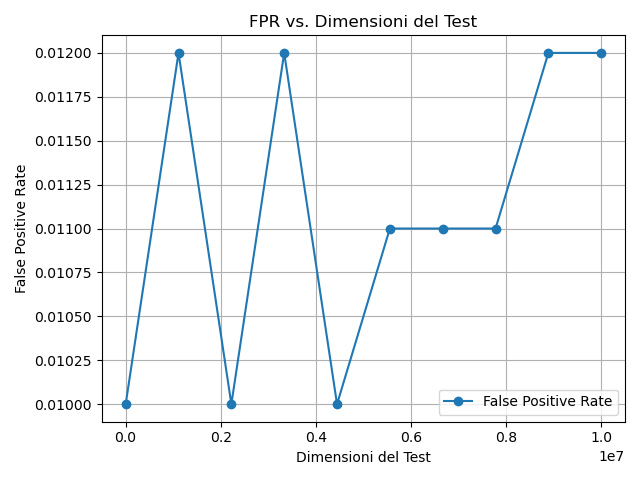
\includegraphics[width=\linewidth]{omp/001/setup_fpr_plot}
            \caption{Speedup setup Omp}\label{fig:setup_fpr_omp}
        \endminipage\hfill
        \minipage{0.49\textwidth}
        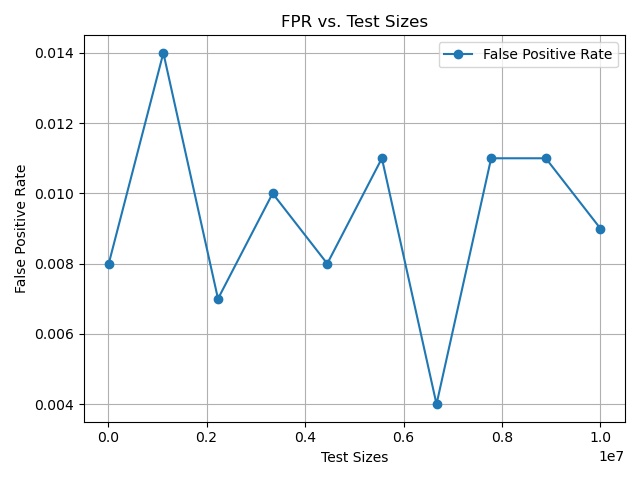
\includegraphics[width=\linewidth]{joblib/001/setup_fpr_plot}
            \caption{Speedup setup Joblib}\label{fig:setup_fpr_joblib}
        \endminipage\hfill
        \caption{Time setup}
    \end{figure}

    \subsubsection{Filter}\label{subsubsec:filter}
    \begin{figure}[H]
        \centering
        \minipage{0.49\textwidth}
        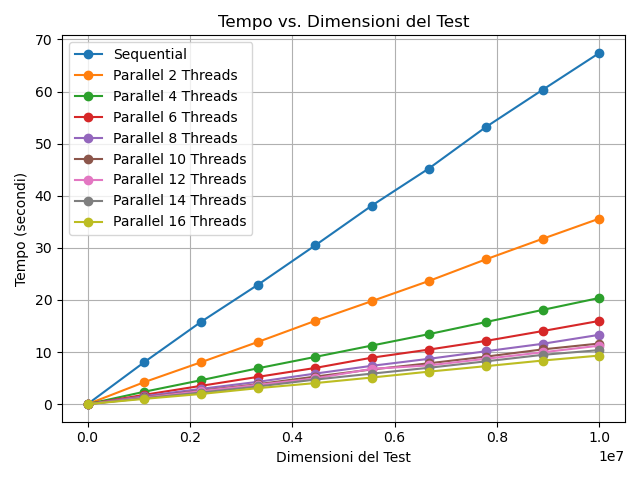
\includegraphics[width=\linewidth]{omp/001/filter_time_plot}
            \caption{Times filter Omp}\label{fig:filter_time_omp}
        \endminipage\hfill
        \minipage{0.49\textwidth}
        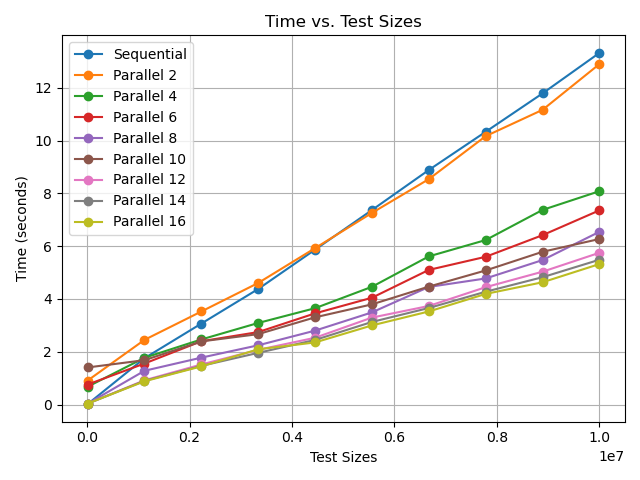
\includegraphics[width=\linewidth]{joblib/001/filter_time_plot}
            \caption{Times filter Joblib}\label{fig:filter_time_joblib}
        \endminipage\hfill
        \caption{Time filter}
    \end{figure}
    \begin{figure}[H]
        \centering
        \minipage{0.49\textwidth}
        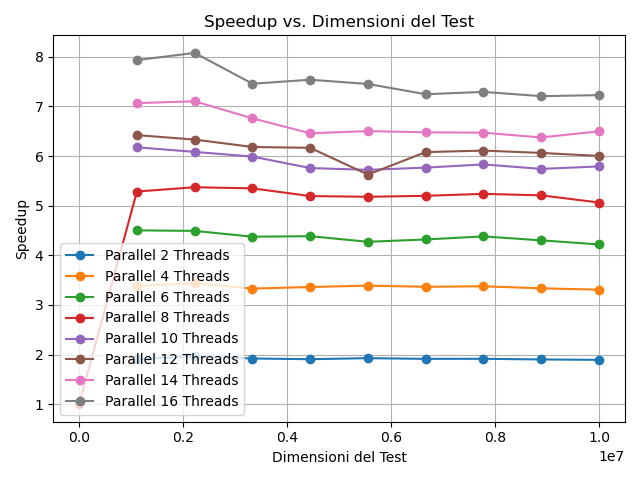
\includegraphics[width=\linewidth]{omp/001/filter_speedup_plot}
            \caption{Speedup filter Omp}\label{fig:filter_speedup_omp}
        \endminipage\hfill
        \minipage{0.49\textwidth}
        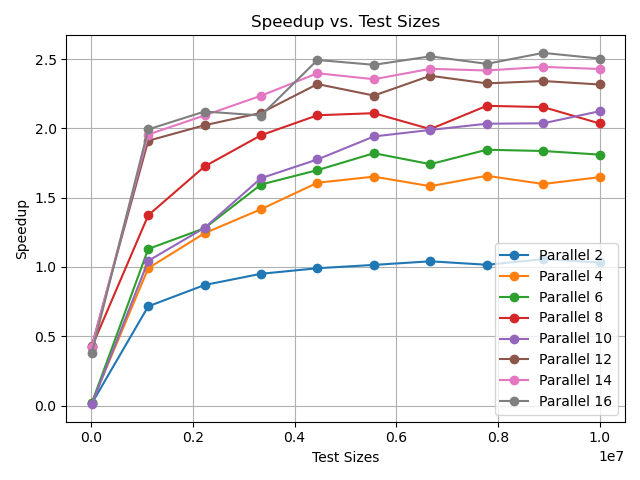
\includegraphics[width=\linewidth]{joblib/001/filter_speedup_plot}
            \caption{Speedup filter Joblib}\label{fig:filter_speedup_joblib}
        \endminipage\hfill
        \caption{Speedup filter}
    \end{figure}
    \begin{figure}[H]
        \centering
        \minipage{0.49\textwidth}
        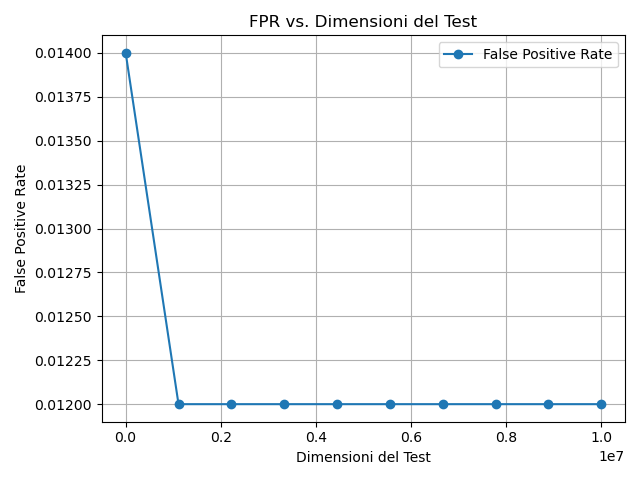
\includegraphics[width=\linewidth]{omp/001/filter_fpr_plot}
            \caption{FPR filter Omp}\label{fig:filter_fpr_omp}
        \endminipage\hfill
        \minipage{0.49\textwidth}
        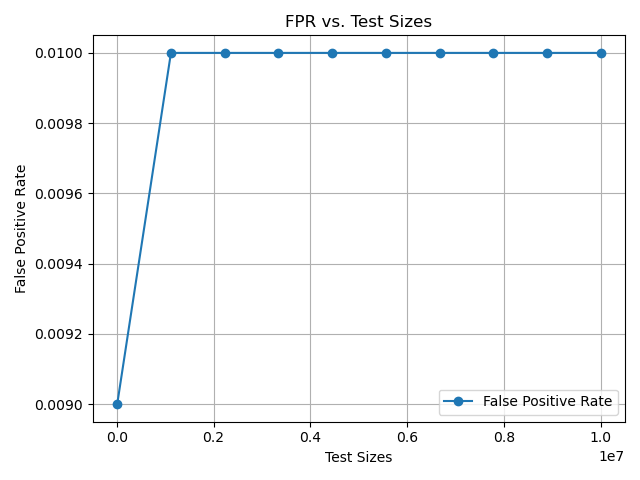
\includegraphics[width=\linewidth]{joblib/001/filter_fpr_plot}
            \caption{FPR filter Joblib}\label{fig:filter_fpr_joblib}
        \endminipage\hfill
        \caption{Time filter}
    \end{figure}

    \subsubsection{Chunks}\label{subsubsec:chunks}
    \begin{figure}[H]
        \centering
        \minipage{0.49\textwidth}
        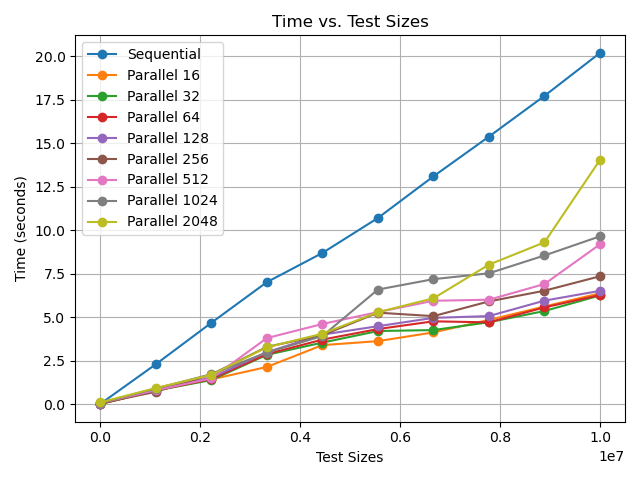
\includegraphics[width=\linewidth]{joblib/001/chunks_time_plot}
            \caption{Times chunks Joblib}\label{fig:chunks_time_joblib}
        \endminipage\hfill
        \minipage{0.49\textwidth}
        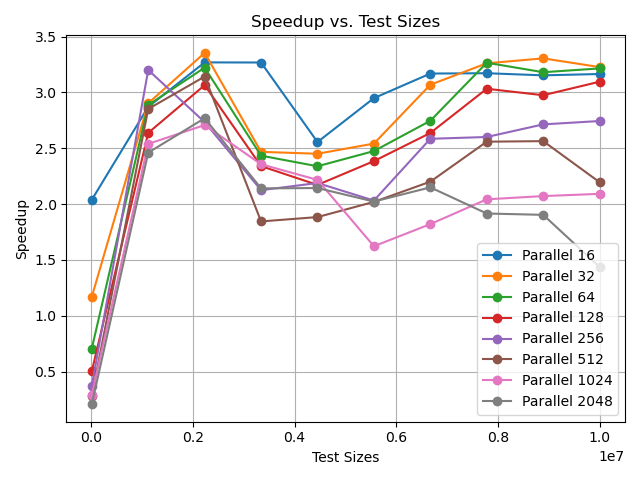
\includegraphics[width=\linewidth]{joblib/001/chunks_speedup_plot}
            \caption{Speedup chunks Joblib}\label{fig:chunks_speedup_joblib}
        \endminipage\hfill
        \caption{Speedup chunks}
    \end{figure}

    \section{Conclusioni}\label{sec:conclusioni}
    Dai risultati ottenuti possiamo vedere come il valore di Speedup massimo si attesti intorno a 3 rispetto alla versione sequenziale.
    In generale possiamo notare come lo speedup aumenti con l'aumentare della dimensione dell'insieme, fino a un certo punto per la versione Joblib.

    \clearpage

    \section{Dati}\label{sec:dati}
    \begin{figure}[H]
        \csvautotabular{../results/csv/setup.csv}\label{fig:setup_csv}
    \end{figure}
    \begin{figure}[H]
        \csvautotabular{../results/csv/filter.csv}\label{fig:filter_csv}
    \end{figure}
    \begin{figure}[H]
        \csvautotabular{../results/csv/chunks.csv}\label{fig:chunks_csv}
    \end{figure}


\end{document}